\documentclass{beamer}
\usepackage[utf8]{inputenc}
\usetheme{Madrid}
\usecolortheme{default}
\usepackage{amsmath,amssymb,amsfonts,amsthm}
\usepackage{txfonts}
\usepackage{tkz-euclide}
\usepackage{listings}
\usepackage{adjustbox}
\usepackage{array}
\usepackage{tabularx}
\usepackage{gvv}
\usepackage{lmodern}
\usepackage{circuitikz}
\usepackage{tikz}
\usepackage{graphicx}

\setbeamertemplate{page number in head/foot}[totalframenumber]

\usepackage{tcolorbox}
\tcbuselibrary{minted,breakable,xparse,skins}



\definecolor{bg}{gray}{0.95}
\DeclareTCBListing{mintedbox}{O{}m!O{}}{%
  breakable=true,
  listing engine=minted,
  listing only,
  minted language=#2,
  minted style=default,
  minted options={%
    linenos,
    gobble=0,
    breaklines=true,
    breakafter=,,
    fontsize=\small,
    numbersep=8pt,
    #1},
  boxsep=0pt,
  left skip=0pt,
  right skip=0pt,
  left=25pt,
  right=0pt,
  top=3pt,
  bottom=3pt,
  arc=5pt,
  leftrule=0pt,
  rightrule=0pt,
  bottomrule=2pt,
  toprule=2pt,
  colback=bg,
  colframe=orange!70,
  enhanced,
  overlay={%
    \begin{tcbclipinterior}
    \fill[orange!20!white] (frame.south west) rectangle ([xshift=20pt]frame.north west);
    \end{tcbclipinterior}},
  #3,
}
\lstset{
    language=C,
    basicstyle=\ttfamily\small,
    keywordstyle=\color{blue},
    stringstyle=\color{orange},
    commentstyle=\color{green!60!black},
    numbers=left,
    numberstyle=\tiny\color{gray},
    breaklines=true,
    showstringspaces=false,
}
%------------------------------------------------------------
%This block of code defines the information to appear in the
%Title page
\title %optional
{1.7.3}

%\subtitle{A short story}

\author % (optional)
{BALU-ai25btech11017}



\begin{document}


\frame{\titlepage}
\begin{frame}{Question}
Show that the points $A(-2\hat{i} + 3\hat{j} + 5\hat{k}), \; 
B(\hat{i} + 2\hat{j} + 3\hat{k}), \; 
\text{and } C(7\hat{i} - \hat{k})$ are collinear.\\ 
\end{frame}



\begin{frame}{Theoretical Solution}

Given positional vectors,
\begin{align}
     \vec{A}=\begin{myvec}{-2\\3\\5}\end{myvec}\;
    \vec{B}=\begin{myvec}{1\\2\\3}\end{myvec}\;
    \vec{C}=\begin{myvec}{7\\0\\-1}\end{myvec}\
\end{align}
To show that these are points are collinear,we show that echolon matrix $\vec{S}$ Rank=1\\

\begin{align}
    \vec{S}=\begin{myvec}{\vec{B}-\Vec{A}&&\vec{C}-\vec{A}}^T\end{myvec}
\end{align}
\begin{align}
     \vec{S}=\begin{myvec}{3&&-1&&-2\\9&&-3&&-6}\end{myvec}
\end{align}


\end{frame}

\begin{frame}{Theoretical Solution}
\begin{align}
By doing R_2=R_2-3R_1 we get \\
   \vec{S}=\begin{myvec}{3&&-1&&-2\\0&&0&&0}\end{myvec}
\end{align}
So the Rank of matrix $\vec{S}$ is 1\\
$\therefore$ The points are collinear.
\end{frame}
\begin{frame}[fragile]
    \frametitle{C Code - Resultant velocity}

    \begin{lstlisting}
#include <stdio.h>

int main() {
    // Points A, B, C
    int Ax = -2, Ay = 3, Az = 5;
    int Bx =  1, By = 2, Bz = 3;
    int Cx =  7, Cy = 0, Cz = -1;

    // Vectors AB = B - A, AC = C - A
    int ABx = Bx - Ax;
    int ABy = By - Ay;
    int ABz = Bz - Az;

    int ACx = Cx - Ax;
    int ACy = Cy - Ay;
    int ACz = Cz - Az;

    printf("Vector AB = (%d, %d, %d)\n", ABx, ABy, ABz);
    
     \end{lstlisting}
\end{frame}
\begin{frame}[fragile]
    \frametitle{C Code - Resultant velocity}

    \begin{lstlisting}
    printf("Vector AC = (%d, %d, %d)\n", ACx, ACy, ACz);
    // Check if AC is a scalar multiple of AB
    // (Cross product must be zero for collinearity)
    int cross_x = ABy * ACz - ABz * ACy;
    int cross_y = ABz * ACx - ABx * ACz;
    int cross_z = ABx * ACy - ABy * ACx;

    printf("Cross product AB x AC = (%d, %d, %d)\n", cross_x, cross_y, cross_z);

    if (cross_x == 0 && cross_y == 0 && cross_z == 0) {
        printf("✅ Points A, B, and C are collinear.\n");
    } else {
        printf("❌ Points A, B, and C are NOT collinear.\n");
    }

    return 0;
}

    \end{lstlisting}
\end{frame}
\begin{frame}[fragile]
    \frametitle{Python Code}
    \begin{lstlisting}
import numpy as np
import matplotlib.pyplot as plt
from mpl_toolkits.mplot3d import Axes3D

# Points
A = np.array([-2, 3, 5])
B = np.array([1, 2, 3])
C = np.array([7, 0, -1])

# Direction vector AB
AB = B - A

# Generate line through A in direction AB
t = np.linspace(-1, 3, 100)  # parameter
line = A[:, None] + AB[:, None] * t





    \end{lstlisting}
\end{frame}

\begin{frame}[fragile]
    \frametitle{Python Code}
    \begin{lstlisting}
# Plot
fig = plt.figure()
ax = fig.add_subplot(111, projection='3d')

# Plot points
ax.scatter(*A, color='red', label='A(-2,3,5)', s=50)
ax.scatter(*B, color='blue', label='B(1,2,3)', s=50)
ax.scatter(*C, color='green', label='C(7,0,-1)', s=50)

# Plot line through A, B, C
ax.plot(line[0], line[1], line[2], color='black', linestyle='--', label='Line through A, B, C')


    \end{lstlisting}
\end{frame}

\begin{frame}[fragile]
    \frametitle{Python Code}
    \begin{lstlisting}


# Labels
ax.set_xlabel('X axis')
ax.set_ylabel('Y axis')
ax.set_zlabel('Z axis')
ax.legend()

# Save figure
plt.savefig("/home/balu/matgeo/figs/fig.png", dpi=300)
plt.show()
    \end{lstlisting}
\end{frame}

\begin{frame}{Plot}
    \centering
    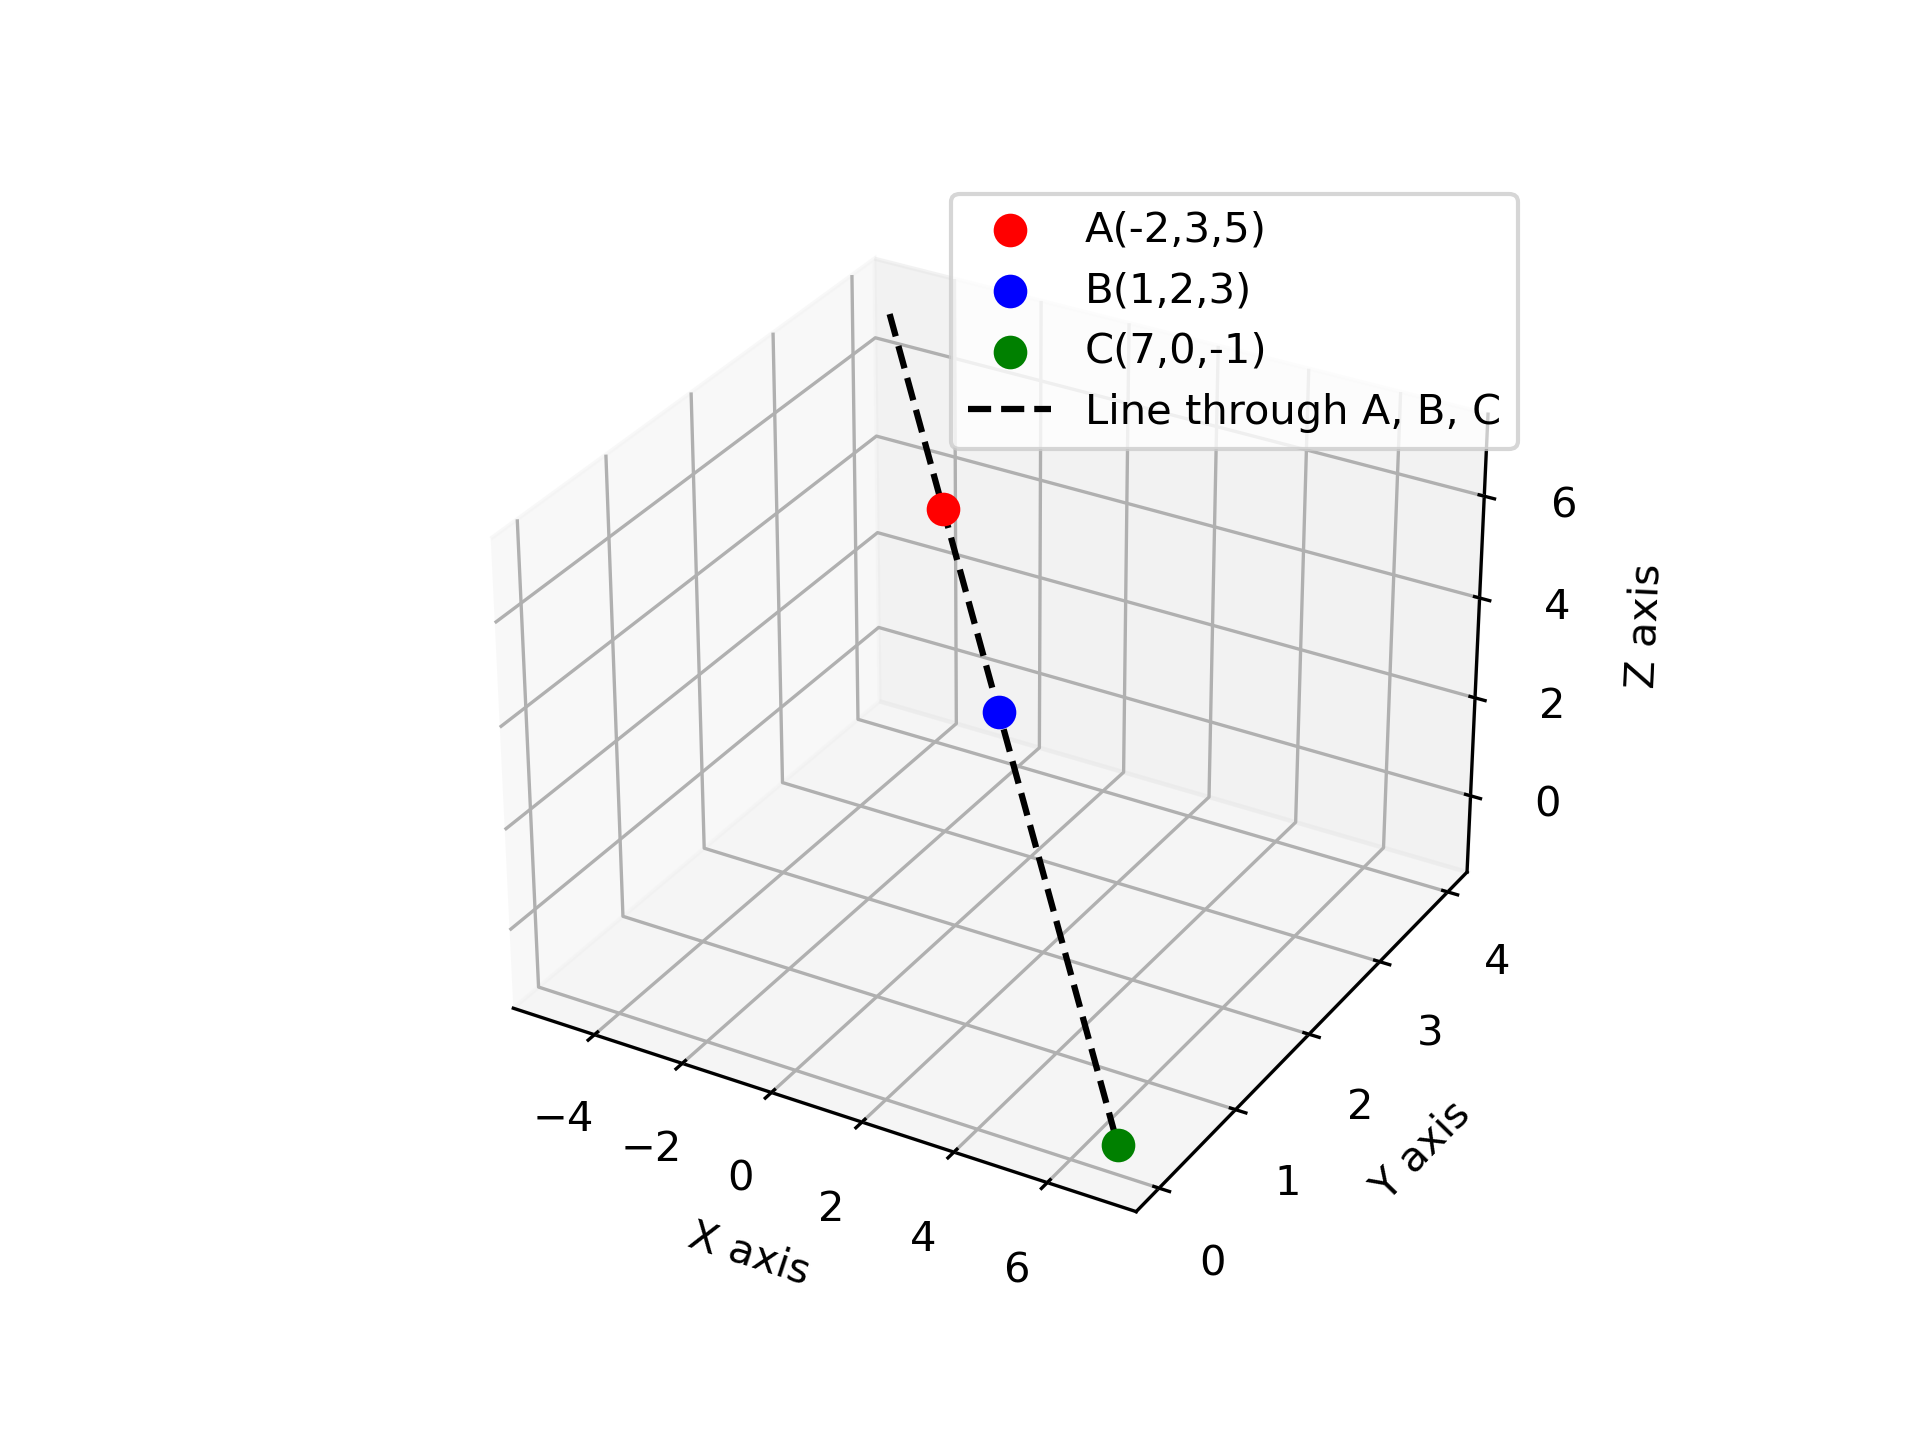
\includegraphics[width=\columnwidth, height=0.8\textheight, keepaspectratio]{figs/fig.png}     
\end{frame}




\end{document}